% Chapter 4

\chapter{Desarrollo}
\label{capitulo4}

\section{Preperaciones del Ambiente de Desarrollo}

\subsection{Sistema Base de Desarrollo}

\begin{figure}
	\begin{center}
    	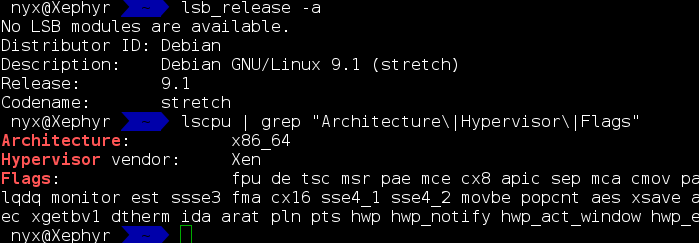
\includegraphics[width=0.75\textwidth]{Figures/sistema-base.png}
    \end{center}
  	\caption{Información del Sistema Base.}
    \label{sistema-base}
\end{figure}

Como se presenta en la figura \ref{sistema-base}, el sistema base para el desarrollo de este trabajo de titulacion utiliza Xen instalado con Debian Stretch (9.1)\footnote{Como el sistema de Dom0} instalado en un LVM con el nombre del grupo de volumenes ''Xephyr-VG''. Originalmente se tenia planificado trabajar con Debian Jessie (8.x) debido que eso fue la version estable al momento de instalacion pero despues se opto por una actualizacion a la version beta de Debian en aquello momento (Debian Stretch). En resumen los pasos realizados fueron:
\lstset{language=Bash}
\begin{enumerate}
	\item Instalacion Limpia de Debian 8 con un LVM.
    	\begin{description}
    		\item[Volumen Fisico:] /dev/sda8 310g 
            \item[Grupo de Volumenes:] Xephyr-VG 310g
            \item[Volumenes Logicos:] Originalmente 4 (se agrega 2 por cada nueva maquina virtual -- uno para su disco y otro para su area de intercambio).
            \begin{description}
            	\item[Xephyr-Dom0] Xephyr-VG 30g
                \item[Xephyr-IMG-Repo] Xephyr-VG 20g
                \item[Xephyr-ISO-Repo] Xephyr-VG 20g
                \item[Xephyr-Swap] Xephyr-VG 4g
            \end{description}
    	\end{description}
    \item Actualizar Instalacion de Debian 8.
    	\begin{lstlisting}
	apt update
	apt upgrade
	apt dist-upgrade
	reboot
        \end{lstlisting}
    \item Actualizar Debian 8 a Debian 9.
        \begin{lstlisting}
	sed -i 's/jessie/stretch/g' /etc/apt/sources.list
	apt update
	apt upgrade
	reboot
        \end{lstlisting}
    \item Instalacion de Herramientas de Trabajo
        \begin{lstlisting}
	apt install tmux vim zsh
        \end{lstlisting}
    \item Instalacion y Configuracion de Hipervisor Xen
		\begin{lstlisting}
	apt install xen-hypervisor
	dpkg-divert --divert /etc/grub.d/08_linux_xen \
		--rename /etc/grub.d/20_linux_xen
	update-grub
	cat > /etc/network/interfaces.d/xenbr << EOF

	auto xenbr0
	iface xenbr0 inet static
		address 10.10.10.1
		netmask 255.255.255.0
		bridge_ports wlan0

	#other possibly useful options in a
	#	virtualized environment
		#bridge_stp off		# disable
		#		Spanning Tree Protocol
		#bridge_waitport 0	# no delay
		#		before a port becomes
		#		available
		#bridge_fd 0		# no forwarding
		#		delay

	## configure a (separate) bridge for
	#	the DomUs without giving Dom0 an
	#	IP on it
	#auto xenbr1
	#iface xenbr1 inet manual
	#   bridge_ports eth1

	EOF

	reboot
		\end{lstlisting}
	\item Instalacion de Herramientas de Xen
		\begin{lstlisting}
	apt install xen-tools xen-utils
		\end{lstlisting}
    \item Instalacion de Herramientas de Desarrollo para Python 3
    	\begin{lstlisting}
	apt install python3 python3-virtualenv python3-pip
    	\end{lstlisting}
    \item Instalacion de Servidores
    	\begin{lstlisting}
	apt install nginx-full postgresql mongodb\
    		redis-server
    	\end{lstlisting}
    \item Instalacion de IDEs en /opt. Se descargaron los respetivos .tar\textit{.xx} y se los descomprimieron en /opt con un comando similar al siguiente:
    	\begin{lstlisting}
	tar -axvf nombre.tar.xx -C\
    		/opt/ruta/raiz/donde/descomprimir
    	\end{lstlisting}
    \begin{enumerate}
    	\item PyCharm (Community o Professional Edition\footnote{Se ocupo una version Professional, en parte por su buen suporte para desarrollo en Django) con una licencia estudiantil que actualmente es gratis de solicitar y renovar año tras año con un correo institucional})
        \item DBeaver (Community o Enterprise Edition\footnote{Historicamente siempre han sido gratis ambas versiones con la diferencia siendo que Enterprise Edition no es completamente software libre a diferencia de su version libre, pero el mismo agrega suporte para bases de datos no relacionales. Se ocupo la version Enterprise, entre los ultimos ofertas gratis antes de que se convierte en un producto de pago, por este mismo motivo de requerir suporte para bases de datos NoSQL como MongoDB y Redis.})
    \end{enumerate}
\end{enumerate}

Estos pasos de instalacion se basaron en la guia de instalacion de Xen publicado en el wiki del proyecto de Debian \citep{Debian-Wiki-Xen}.

Para dar connexiones hace el exterior a las maquinas virtuales, se necesita activar una regla NAT en el cortafuego IPTables:

\begin{lstlisting}
	iptables -t nat -A POSTROUTING -o wlan0\
    		-j MASQUERADE
\end{lstlisting}

\subsection{Ambiente Virtual de LMS (Moodle)}
\label{instalacion-moodle}

Para el ambiente de Moodle (LMS contra el cual se ha llevado el desarrollo), se crea una maquina virtual de Debian Stretch (9) con 1 GiB de RAM, 1 CPU virtual, 6 GiB de disco, 512 MiB de intercambio y una direccion IP fija de 10.10.10.10. Los resultados del mismo commando se puede ver en la figura \ref{vm-moodle}.
\begin{lstlisting}
	xen-create-image --hostname=debian-moodle\
    		--ip=10.10.10.10 --netmask=255.255.255.0\
        	--gateway=10.10.10.1 --memory=1024mb\
        	--vcpus=1 --lvm=Xephyr-VG --pygrub\
        	--dist=stretch --force --size=6144mb\
        	--swap=512mb
\end{lstlisting}

\begin{figure}
	\begin{center}
    	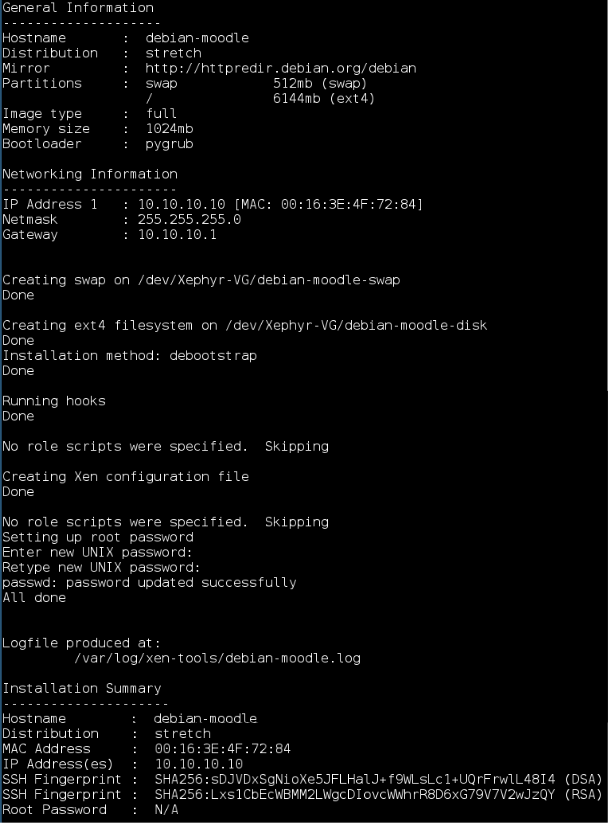
\includegraphics[width=0.75\textwidth]{Figures/crear-moodle.png}
    \end{center}
  	\caption{Crear maquina virtual para Moodle.}
    \label{vm-moodle}
\end{figure}

Se renombró el archivo de configuracion de la maquina virtual generado en el paso anterior para temas de consistencia.

\begin{lstlisting}
	mv /etc/xen/debian-moodle.cfg\
    		/etc/xen/domU-debian-moodle.cfg
\end{lstlisting}

Un bug de Xen-Tools causa que no se instala correctamente un nucleo de Linux en la maquina virtual y por lo tanto es necesario entrar al mismo con un Chroot y instalar los paquetes faltantes (y hacer las adecuadas configuraciones  para permitir su aranque independiente de ayuda externa).

\begin{lstlisting}
	mount /dev/Xephyr-VG/debian-moodle-disk /mnt
	mount -o bind /proc /mnt/proc
	mount -o bind /sys /mnt/sys
	mount -o bind /dev /mnt/dev
	cp /etc/resolv.conf /mnt/etc/resolv.conf
	chroot /mnt /bin/bash
	apt install linux-image-amd64
	vim.tiny /boot/grub/menu.lst
	# Revisar que los archivos referenciados existen
	#		de verdad por ejemplo:
	# Replace initrd.img- con initrd.img
    # guarda y sale
	exit
	umount /mnt/proc            
	umount /mnt/sys 
	umount /mnt/dev 
	umount /mnt	
\end{lstlisting}

Para levantar la maquina virtual:

\begin{lstlisting}
	xl create /etc/xen/domU-debian-moodle.cfg -c
\end{lstlisting}

Se debe selecionar la tercera opcion (Default Kernel).

Se puede dar una revision a la configuracion de red para asegurarse de que esta correcto:

\begin{lstlisting}
	vim.tiny /etc/network/interfaces
\end{lstlisting}

Debe contener:

\begin{lstlisting}
auto eth0
iface eth0 inet static
 address 10.10.10.10
 gateway 10.10.10.1
 netmask 255.255.255.0
\end{lstlisting}

En el presente caso, Xen-Tools logró configurar esta parte de forma correcta.

A continuacion se procede con la instalacion de Moodle:

\begin{lstlisting}
# actualiza el sistema
apt update
apt upgrade

# instala dependencias
apt install apache2 php7.0 mysql-server php7.0-mysql
apt install libapache2-mod-php7.0 php7.0-gd php7.0-curl
apt install php-xml php-zip php-mbstring php-soap
apt install php7.0-xmlrpc php7.0-intl
vim.tiny /etc/php/7.0/apache2/php.ini

# agrega:
extension=mysql.so 
extension=gd.so

# edita:

memory_limit = 40M
# dejado con el valor por defecto de 128M

post_max_size = 80M
upload_max_filesize = 80M

# guarda y sale

# reinicia apache para coger los cambios
systemctl restart apache2

\end{lstlisting}

A continuacion se configura la base de datos:

\begin{lstlisting}

# clave de root es root
mysqladmin -u root password "root"

# logear como root
mysql -u root -p

# crear base de datos y hacer que ocupa UTF-8
mysql> CREATE DATABASE moodle;
mysql> ALTER DATABASE moodle charset=utf8;
mysql> exit;

## No se implemento ##
# Moodle queja de UTF8

# Se podria arreglar
# (antes de instalar Moodle)
# con:

mysql -u root -p

mysql> ALTER DATABASE moodle charset=utf8mb4;
mysql> exit;
######################

systemctl restart mysql

\end{lstlisting}

Se realiza la instalacion de la ultima version de Moodle (3.3 con sus respectivos patches de fallas desde que el mismo salio):

\begin{lstlisting}

# descargar
wget https://download.moodle.org/download.php/direct/stable33/moodle-latest-33.tgz

# descomprimir
tar -zxvf moodle-latest-33.tgz

# meter en ubicacion para apache
mv moodle /var/www

# ir a ubicacion para apache
cd /var/www

# crear ubicacion para datos
mkdir moodledata

# arreglar permisos
chown -R www-data:www-data moodle
chown -R www-data:www-data moodledata
chmod -R 755 moodle
chmod -R 755 moodledata

# modificar configuracion de apache
vim.tiny /etc/apache2/sites-available/000-default.conf

# editar
DocumentRoot "/var/www/moodle"

# guardar y salir

# reiniciar apache para aplicar los cambios
systemctl restart apache2

\end{lstlisting}

Arreglar la base de datos para que acepte conexiones desde Moodle:

\begin{lstlisting}

mysql -u root -p

GRANT ALL PRIVILEGES on *.* to
	'root'@'localhost' IDENTIFIED BY 'root';
GRANT ALL PRIVILEGES on *.* to
	'root'@'localhost' IDENTIFIED BY 'root';
FLUSH PRIVILEGES;
exit;

\end{lstlisting}

Para seguir con la instalacion se abre un navegador con la direccion \url{http://10.10.10.10/} para seguir las instrucciones que se le lleve por toda la configuracion inicial del Moodle.

Al final se agrege un trabajo de cron para ayudar con los tareas periodicas que Moodle requiere para su mantemiento continuo:

\begin{lstlisting}

crontab -u www-data -e
# add line:
*/10 * * * * /usr/bin/php
		/var/www/moodle/admin/cli/cron.php
        		>/dev/null

\end{lstlisting}

Estos pasos fueron adaptados de la guia oficial del proyecto de Moodle para instalacion en Debian \citep{MOODLE-Install-Debian}.

Ahora que todo esta funcionando se recomienda editar /boot/grub/menu.lst para comentar las entradas del pyGrub que son defectuosas (los primeros dos) para que se puede levantar la maquina virtual sin intervencion humana.

\subsection{Servidor de Git (GitLab CE)}
Para crear el servidor de Git con GitLab Community Edition, se va a empezar con las mismas piezas del servidor del LMS/Moodle, es decir una maquina virtual de Debian 9. El mismo se crea como una maquina virtual de Debian Stretch (9) con 1 GiB de RAM, 1 CPU virtual, 6 GiB de disco, 512 MiB de intercambio y una direccion IP fija de 10.10.10.11.
\begin{lstlisting}
	xen-create-image --hostname=debian-gitlab\
    		--ip=10.10.10.11 --netmask=255.255.255.0\
        	--gateway=10.10.10.1 --memory=1024mb\
        	--vcpus=1 --lvm=Xephyr-VG --pygrub\
        	--dist=stretch --force --size=6144mb\
        	--swap=512mb
\end{lstlisting}

Se renombró el archivo de configuracion de la maquina virtual generado en el paso anterior para temas de consistencia.

\begin{lstlisting}
	mv /etc/xen/debian-gitlab.cfg\
    		/etc/xen/domU-debian-gitlab.cfg
\end{lstlisting}

Un bug de Xen-Tools causa que no se instala correctamente un nucleo de Linux en la maquina virtual y por lo tanto es necesario entrar al mismo con un Chroot y instalar los paquetes faltantes (y hacer las adecuadas configuraciones  para permitir su aranque independiente de ayuda externa).

\begin{lstlisting}
	mount /dev/Xephyr-VG/debian-gitlab-disk /mnt
	mount -o bind /proc /mnt/proc
	mount -o bind /sys /mnt/sys
	mount -o bind /dev /mnt/dev
	cp /etc/resolv.conf /mnt/etc/resolv.conf
	chroot /mnt /bin/bash
	apt install linux-image-amd64
	vim.tiny /boot/grub/menu.lst
	# Revisar que los archivos referenciados existen
	#		de verdad por ejemplo:
	# Replace initrd.img- con initrd.img
    # guarda y sale
	exit
	umount /mnt/proc            
	umount /mnt/sys 
	umount /mnt/dev 
	umount /mnt	
\end{lstlisting}

Para levantar la maquina virtual:

\begin{lstlisting}
	xl create /etc/xen/domU-debian-gitlab.cfg -c
\end{lstlisting}

Se debe selecionar la tercera opcion (Default Kernel).

Se puede dar una revision a la configuracion de red para asegurarse de que esta correcto:

\begin{lstlisting}
	vim.tiny /etc/network/interfaces
\end{lstlisting}

Debe contener:

\begin{lstlisting}
auto eth0
iface eth0 inet static
 address 10.10.10.11
 gateway 10.10.10.1
 netmask 255.255.255.0
\end{lstlisting}

En el presente caso, Xen-Tools logró configurar esta parte de forma correcta.

A continuacion se procede con la instalacion de Gitlab:

\begin{lstlisting}
# actualiza el sistema
apt update
apt upgrade

# Apartir del Debian 9, Gitlab CE esta ofrecido
#    en los repositorios oficiales:
apt install gitlab

# Arreglar problema con API
vim.tiny /usr/share/gitlab-shell/config.yml
# cambiar gitlab_url a "http://10.10.10.11/"

/usr/share/gitlab-shell/bin/check
\end{lstlisting}

Visitar \url{http://10.10.10.11/} y configurar la contraseña del usuario root. Con el usuario root configurado se procede a crear un usuario especial para la aplicacion con el nombre de usuario 'GitEdu'. Este usuario lo damos permisos de administracion y tambien se genera un token en esta direccion: \url{http://10.10.10.11/profile/personal_access_tokens}. El token se debe guardar para su uso despues (GitLab nunca le vuelve a mostrar).

Ahora que todo esta funcionando se recomienda editar /boot/grub/menu.lst para comentar las entradas del pyGrub que son defectuosas (los primeros dos) para que se puede levantar la maquina virtual sin intervencion humana.

% <TODO>

%%%%%%%%%%%%%%%%%%%%%%%%%%%%%%%%%%%%%%%%%%%%%%%%%%%%
% \subsection{Servidor de Virtualizacion (???)}
%%%%%%%%%%%%%%%%%%%%%%%%%%%%%%%%%%%%%%%%%%%%%%%%%%%%

%%%%%%%%%%%%%%%%%%%%%%%%%%%%%%%%%%%%%%%%%%%%%%%%%%%%
% \subsection{Plantilla de Maquina Virtual (???)}
%%%%%%%%%%%%%%%%%%%%%%%%%%%%%%%%%%%%%%%%%%%%%%%%%%%%

% </TODO>

\section{GitEDU}

La gestion de dependencias del sistema GitEdu se maneja con un entorno virtual y el gestor de paquetes de python pip. El siguiente es un script de bash diseñado a detectar si es que existe el entorno virtual (lo crea en caso de que no existe) y despues instala los requiermientos faltantes como son especificados en un archivo aparte ''requirements.txt'' que da liberias y sus versiones.

\begin{lstlisting}

# run with `source activate.sh` 
if [ ! -d env ]; then
	virtualenv --python=python3 env
fi
source env/bin/activate
pip3 install -r requirements.txt

\end{lstlisting}

El script anterior se ejecuta desde el raiz del repositorio con el comando:

\begin{lstlisting}
source activate.sh
\end{lstlisting}

Con el entorno creado y activado se puede proceder a instalar cualquier dependencia necesaria que no ha sido instalado previamente:

\begin{lstlisting}
pip install <nombre_dependencia>
\end{lstlisting}

Para el presente proyecto se instalaron las siguientes dependencias:
\begin{itemize}
	\item Django (1.10.6) como framework para el desarrollo del backend.
    \item Psycopg2 (2.7.1) como liberia para connectarse a bases de datos PostgreSQL.
    \item Python-GitLab (0.20) como liberia para consumir el API de GitLab.
\end{itemize}

Con las dependencias instaladas o con cada cambio que se realiza de dependencias se ejecuta el siguiente commando para actualizar la lista de los mismos:

\begin{lstlisting}
pip freeze > requirements.txt
\end{lstlisting}

Tambien antes de iniciar el desarrollo debe estar configurado el base de datos para ocupar el mismo. Primero es necesario crear y configurar un usuario y base de datos para ser ocupado:
\begin{lstlisting}
postgresql-setup initdb
systemctl enable postgresql
systemctl start postgresql
systemctl status postgresql
vim /etc/postgresql/9.6/main/pg_hba.conf
# agregar una linea antes de las lineas similares y
# que diga (sin el numeral adelante):
#local   all      postgres             peer
systemctl restart postgresql
systemctl status postgresql
su - postgres
psql
\end{lstlisting}
\begin{lstlisting}
	postgres=# CREATE USER giteduser WITH PASSWORD 'g1T3d_$3r';
	postgres=# CREATE DATABASE gitedudb WITH OWNER giteduser;
	postgres=# \q
psql gitedudb -U postgres
	gitedudb=# CREATE SCHEMA giteduapp AUTHORIZATION giteduser;
	gitedudb=# ALTER USER giteduser SET search_path TO giteduapp;
	gitedudb=# \q
psql gitedudb -U giteduser
	gitedudb=> SELECT current_schema();
		Debe decir: giteduapp
	gitedudb=> \q
\end{lstlisting}

Segundo, se abre el settings.py (dentro de la carpeta GitEDU/GitEDU) y se remplaza (para desarrollo, en produccion debe llevar valores distintos) el atributo DATABASES con lo siguiente:
\lstset{language=Python}
\begin{lstlisting}
DATABASES = {
    'default': {
        'ENGINE': 'django.db.backends.postgresql_psycopg2',
        'NAME': 'gitedudb',
        'USER': 'giteduser',
        'PASSWORD': 'g1T3d_$3r',
        'HOST': '127.0.0.1',
        'PORT': '5432',
    }
}
\end{lstlisting}
\lstset{language=Bash}

Ahora se puede migrar las tablas iniciales de Django:
\begin{lstlisting}
cd GitEDU
python manage.py makemigrations
python manage.py migrate
\end{lstlisting}

Tambien creamos un superusuario de Django para temas administrativos:
\begin{lstlisting}
python manage.py createsuperuser
\end{lstlisting}

Tambien se puede crear el app inicial (para logica del editor de codigo):
\begin{lstlisting}
python manage.py startapp ideApp
\end{lstlisting}

Y de paso se lo agrega a INSTALLED\_APPS una linea 'ideApp' en el settings.py para que sus tablas definidos a futuro en models.py tambien se migran con los demas migraciones.

Para resolver un problema de zonas de tiempo, se ha deactivado esta caracteristica de Django con el siguiente linea en el settings.py:
\lstset{language=Python}
\begin{lstlisting}
USE_TZ = False
\end{lstlisting}
\lstset{language=Bash}

Para crear la base de datos de MongoDB:
\begin{lstlisting}
mongo
\end{lstlisting}
\lstset{language=sql}
\begin{lstlisting}
use gitEduDB
db.createUser(
    {
        user: "gitEduUser",
        pwd: "G1TedU$3r",
        roles: [ "readWrite", "dbAdmin" ]
    }
)
\end{lstlisting}
\lstset{language=Bash}

El mismo se define en el settings de la siguiente manera:
\lstset{language=Python}
\begin{lstlisting}
NOSQL_DATABASES = {
    'nosql': {
        'NAME': 'gitEduDB',
        'USER': "gitEduUser",
        'PASSWORD': 'G1TedU$3r',
        'HOST': '127.0.0.1',
        'PORT': '27017',
    }
}
\end{lstlisting}
\lstset{language=Bash}

\subsection{Autenticacion Clasica}

Primero se crea una nueva aplicacion para autenticacion clasica:
\begin{lstlisting}
python manage.py startapp authApp
\end{lstlisting}

Y de paso se lo agrega a INSTALLED\_APPS una linea 'authApp' en el settings.py para que sus tablas definidos a futuro en models.py tambien se migran con los demas migraciones.

Para la implementacion de autenticacion clasica, se reutilizo el modulo con el mismo proposito del proyecto anterior GitEduERP. A esta se aumento la funcionalidad adcional de que desde el settings se puede activar o desactivar la funcionalidad de permitir a usuarios registrarse a traves del atributo ENABLE\_REGISTRATION. 

Para el registro de usuarios, se considera que solo debe permitirse (en caso de que sea habilitado por la administacion) el registro de estudiantes y docentes pero no de administradores, motivo por el cual se ha considerado duplicar los formularios de registro y ofrecer uno para estudiantes y otro para docentes. Los mismos se pueden habilitar y deshabilitar con los atributos ENABLE\_STUDENT\_REGISTRATION y ENABLE\_TEACHER\_REGISTRATION respectivamente.

\subsection{Autenticacion por LTI}

Primero es necesario que este activo y levantado el ambiente del LMS como se documenta en la seccion \ref{instalacion-moodle} de instalacion de Moodle. Para el desarrollo de este trabajo de titulacion se esta considerando una instalacion en un servidor aparte (virtualizado en el mismo equipo) en la direccion IP 10.10.10.10.

% Instalar dependencias

Instalacion de dependencias desde GitHub (no se encuentran en los repositorios oficiales de Pip/Pypi; ademas para superar problemas de dependencias en las librerias, se ha optado para ocupar forks personales del autor con las mejores necesarias para su funcionamiento):
\begin{lstlisting}
pip install git+https://github.com/nishedcob/django-app-lti
	@master#egg=django-app-lti
pip install git+https://github.com/nishedcob/
	django-auth-lti@master#egg=django-auth-lti
\end{lstlisting}

Como son dependencias no se encuentran en los repositorios oficiales, su manejo dentro del requirements.txt tambien tiene que ser especial ya que un `pip freeze` no los guardaran correctamente dentro del mismo. En lugar de eso hay que agregar dos lineas al requirements.txt para el manejo de estas dependencias:
\begin{lstlisting}
-e git+https://github.com/nishedcob/django-app-lti.git
	@38b32989e22b189345e421b183684f9b5453e99a
	#egg=django-app-lti
-e git+https://github.com/nishedcob/django-auth-lti.git
	@71c9da8d0aa07ebc3139bf3f113b5c521d61b1f1
	#egg=django-auth-lti
\end{lstlisting}

% Modificar settings

\lstset{language=Python}

Se pone a editar el settings.py (dentro de GitEDU/GitEDU) con las siguientes configuraciones:
\begin{itemize}
	\item a INSTALLED\_APPS agregamos las siguientes lineas:
   		\begin{lstlisting}
    'django_auth_lti',
    'django_app_lti',
    	\end{lstlisting}
    \item a MIDDLEWARE agregamos la siguiente linea:
   		\begin{lstlisting}
    'django_auth_lti.middleware.LTIAuthMiddleware',
    	\end{lstlisting}
    \item a AUTHENTICATION\_BACKENDS agregamos la siguiente linea:
   		\begin{lstlisting}
    'django_auth_lti.backends.LTIAuthBackend',
    	\end{lstlisting}
        Si es que no existe AUTHENTICATION\_BACKENDS lo creamos con los siguientes valores:
        \begin{lstlisting}
AUTHENTICATION_BACKENDS = (
    'django.contrib.auth.backends.ModelBackend',
    'django_auth_lti.backends.LTIAuthBackend',
)
        \end{lstlisting}
    \item tambien agregamos los siguientes atributos:
    	\begin{itemize}
    		\item LTI\_SETUP
            	\begin{lstlisting}
LTI_SETUP = {
    "TOOL_TITLE": "GitEDU",
    "TOOL_DESCRIPTION": "Sistema para Programar en Linea",
    "LAUNCH_URL": "lti:launch",
    "LAUNCH_REDIRECT_URL": "ideApp:decode",
    "INITIALIZE_MODELS": False,
    "EXTENSION_PARAMETERS": {
        "10.10.10.10": {
            "privacy_level": "public",
            "course_navigation": {
                "enabled": "true",
                "default": "disabled",
                "text": "GitEDU LMS Playground",
            }
        }
    }
}
            	\end{lstlisting}
            \item LTI\_OAUTH\_CREDENTIALS con texto aleatorio (fue ocupado OpenSSL, especificamente el commando \texttt{openssl rand -hex 10} para generar los valores de abajo\footnote{Un ambiente de produccion debe ocupar valores distintos}).
            	\begin{lstlisting}
LTI_OAUTH_CREDENTIALS = {
    "GitEduLMS_Playground": "b2e0158c3cb4ddb0202d", 
         # (Para pruebas)
    "GitEduLMS_Playground_Assignments":
         "57b3a14734566c49bcaf",
         # (Para deberes/examenes/pruebas/talleres/etc)
    "GitEduLMS_Playground_Classes":
         "f7a0b6accc2631779e84",
         # (Para materias)
}
            	\end{lstlisting}
    	\end{itemize}
\end{itemize}

Tambien se edita el urls.py (dentro de la misma direccion que el settings.py) con las siguientes lineas:
\begin{lstlisting}
from django.conf.urls import include
import django_app_lti.urls

# dentro de:
urlpatterns = [
    # agregar:
    url(r'^lti/', include(django_app_lti.urls, namespace="lti")),
]

\end{lstlisting}

\lstset{language=Bash}

Para arreglar un problema de una version muy desactualizada de ims-lti-py, se agrego la siguiente linea al requirements.txt (para ocupar un fork del propio liberia por el propio autor para resolver los problemas dados):
\begin{lstlisting}
-e git+https://github.com/nishedcob/ims_lti_py.git
	@a6576d7892ea4f69b76572788b118aaa4cdcf749
	#egg=ims_lti_py-develop
\end{lstlisting}

Para arreglar un problema de limpieza de datos en oauth2, se agrego la siguiente linea al requirements.txt (para ocupar un fork del propio liberia por el propio autor para resolver los problemas dados):
\begin{lstlisting}
-e git+https://github.com/nishedcob/python-oauth2.git
	@176fc35aa35d626afcb6a23459482a4c96782c88
	#egg=oauth2
\end{lstlisting}

Despues se migra la base de datos:
\begin{lstlisting}
python manage.py makemigrations
python manage.py migrate
\end{lstlisting}

\subsubsection{Validacion}

Se levanta la aplicacion (en \url{http://localhost:8000/} con:
\begin{lstlisting}
python manage.py runserver
\end{lstlisting}
La maquina virtual de Moodle tambien debe estar levantado para navegar a \url{http://10.10.10.10/}, iniciarse session como administrador, ir a la parte administrativa, a la pestaña de ''development'', seleccionar ''debugging'', y poner ''debug messages'' a nivel ''developer''. Ahora podemos volver a la parte de administracion, volver a seleccionar la pestaña de ''development'' y crear un curso de prueba. Vamos a crear un curso pequeña (10 MB) con el nombre corto ''Prog\_I'' y nombre larga / descripcion ''Introduccion a la Programacion''. Una vez que nos carga el curso, activamos modo de editar y agregamos una actividad externa.

Se da un nombre a la actividad, en este caso ''Prueba 1 Programacion''. La mejor forma de poder reutilizar la herramienta externa en varias actividades es de crear una herramienta ''Preconfigurada''. Las opciones elegidas para la misma fueron los siguientes:
\begin{description}
	\item[Nombre] GitEdu
    \item[URL] \url{http://localhost:8000/lti/launch}
    \item[Descripcion] Edit Code Online
    \item[Llave de Consumidor] GitEduLMS\_Playground
    \item[Secreto Compartido] b2e0158c3cb4ddb0202d
    \item[Parametros Addicionales] lo dejamos en blanco
    \item[Contenedor de Lanzamiento] Nueva ventana
    \item[Compartir Nombre] Siempre
    \item[Compartir Correo Electronico] Siempre
    \item[Acceptar Notas] Siempre
\end{description}
Con la herramienta preconfigurada realizada, se puede selecionarlo asi no mas para completar la integracion. Donde se creó la actividad debe haber un enlace con el nombre del mismo, en este caso ''Prueba 1 Programacion''. Al abrir el enlace se debe llevar a la aplicacion con lo siguiente puntos interesantes:
\begin{enumerate}
	\item se encuentra autenticado con el mismo usuario de Moodle (incluyendo sus roles como ''administrador'', ''instructor'', ''estudiante'', etc\ldots{})
    \item hay contexto de:
    \begin{enumerate}
    	\item el curso de origen de Moodle
        \item la actividad de origen de Moodle (no es contexto completo, un problema que se tendra que resolver en el curso del desarrollo)
        \item el llave de consumidor ocupado
    \end{enumerate}
\end{enumerate}

Si, dentro del mismo curso creamos una segunda actividad con todo lo mismo, pero solo cambiando el nombre a ''Prueba 2 Programacion'', se encuentra que si logra distinguir entre actividades.

\subsection{Integracion de Dos Schemas de Autenticacion}
Los dos schemas de autenticacion implemententadas, sea la forma clasica con nombre de usuario y contraseña corespondiente o por LTI donde una aplicacion externa autentica un usuario autenticado previamente por el mismo, tienen un mismo fin de permitir que el sistema conozca quien esta accediendo el sistema con un fin de dar el comportamiento adecuado y en base a ello proveer seguridad y funcionalidad adecuado a todos los usuarios segun su rol.

Para el mismo se propone tres tablas en la base de datos expresados como modelos de Django:
\lstset{language=Python}
\begin{lstlisting}
class EquivalentUser(models.Model):
    normal_user = models.ForeignKey(auth_models.User,
                                    on_delete=models.CASCADE,
                                    related_name=
                                      "equivalent_normal_user",
                                    null=False)
    lti_user = models.ForeignKey(auth_models.User,
                                 on_delete=models.CASCADE,
                                 related_name=
                                   "equivalent_lti_user",
                                 null=False)

    def __str__(self):
        return "EqU: %s = %s" % (self.normal_user.username,
                                 self.lti_user.username)


class AuthenticationType(models.Model):
    name = models.CharField(max_length=50, unique=True,
                            null=False)

    def __str__(self):
        return "AuT: %s" % self.name


class UserAuthentication(models.Model):
    authentication_type = models.ForeignKey(AuthenticationType,
                                            null=False,
                                            on_delete=
                                              models.CASCADE)
    user = models.ForeignKey(auth_models.User, on_delete=
                                                 models.CASCADE,
                             null=False)

    def __str__(self):
        return "UAuTy: %s - %s" % (self.user.username, 
                                   self
                                     .authentication_type
                                     .name)
\end{lstlisting}
\lstset{language=Bash}
La tabla EquivalentUser relaciona usuarios autenticados de forma clasica con usuarios autenticados por LTI (porque por cada metodo de autenticacion se cree un nuevo usuario para su propio uso interno) con un fin de permitir relacionar distintos usuarios dentro del sistema quienes representan el mismo individuo natural. El idea es por ejemplo, si un docente se autentica por LTI y tambien por usuario y contraseña, para el sistema esta ocupando dos usuarios diferentes pero para el docente esta accediendo el mismo sistema y por lo tanto el comportamiento del sistema, sin tomar en cuenta como se autentica, debe ser igual y debe tener acceso a los mismos contenidos. La tabla AuthenticationType es un catalogo de formas de autenticacion que suporta el sistema y por su naturaleza de catalogo se llena con las migraciones. Y finalmente la tabla UserAuthentication documenta el tipo de autenticacion asociado con un usuario para dar el contexto al sistema que necesita para manejar distintos datos de los diferentes tipos de usuarios.

Con una migracion se puede llenar de forma automatica el catalogo de AuthenticacionType:
\lstset{language=Python}
\begin{lstlisting}
def fill_auth_types(apps, schema_editor):
    auth_type = models.AuthenticationType
    classic = auth_type(name="Clasica")
    classic.save()
    lti = auth_type(name="LTI")
    lti.save()


class Migration(migrations.Migration):

    dependencies = [
        ('authApp',
           '0002_authenticationtype_userauthentication'),
    ]

    operations = [
        migrations.RunPython(fill_auth_types),
    ]
\end{lstlisting}
\lstset{language=Bash}

\subsection{Accesibilidad a Datos de Autenticacion de LTI}
Primero al settings se agrega dos atributos que indiquen cual llave se considera el sistema para compartir materias y otro para compartir deberes/examenes/pruebas/talleres/etc\ldots{}:
\lstset{language=Python}
\begin{lstlisting}
LTI_ASSIGNMENTS_KEY = 'GitEduLMS_Playground_Assignments'
LTI_CLASSES_KEY = 'GitEduLMS_Playground_Classes'
\end{lstlisting}
\lstset{language=Bash}

Para controlar las partes de la configuracion que se presenta a los usuarios finales, agregamos un nuevo campo de configuracion al settings:
\lstset{language=Python}
\begin{lstlisting}
LTI_CONFIG_EXPOSE = {
    "LTI_KEYS": True,
    "LTI_ASSIGNMENT_KEY": True,
    "LTI_CLASS_KEY": True,
    "LTI_OTHER_KEYS": False,
    "LTI_SETUP": False,
}
\end{lstlisting}
\lstset{language=Bash}

Para que los professores (como usuario final de GitEdu) tambien tengan acceso a estos credenciales para poderlos ocupar, se cree una vista en la ubicacion '/auth/lti/credentials' que devuelve un JSON con los datos de LTI:
\lstset{language=Python}
\begin{lstlisting}
class LTICredentialsView(View):

    def get(self, request):
        if not request.user.is_authenticated:
            raise PermissionError("No tiene acceso a esta\
                vista hasta que se autentica...")

        lti_expose = settings.LTI_CONFIG_EXPOSE

        lti_cred_json = {}

        if lti_expose['LTI_KEYS']:
            if lti_expose['LTI_ASSIGNMENT_KEY']:
                lti_cred_json['LTI_ASSIGNMENT_KEY'] = {
                    settings.LTI_ASSIGNMENTS_KEY: 
                        settings.LTI_OAUTH_CREDENTIALS
                            [settings.LTI_ASSIGNMENTS_KEY]
                }
            if lti_expose['LTI_CLASS_KEY']:
                lti_cred_json['LTI_CLASS_KEY'] = {
                    settings.LTI_CLASSES_KEY:
                        settings.LTI_OAUTH_CREDENTIALS
                            [settings.LTI_CLASSES_KEY]
                }
            if lti_expose['LTI_OTHER_KEYS']:
                lti_cred_json['LTI_OTHER_KEYS'] =
                    settings.LTI_OAUTH_CREDENTIALS

        if lti_expose['LTI_SETUP']:
            lti_cred_json['LTI_SETUP'] =
                settings.LTI_SETUP

        return JsonResponse(lti_cred_json)
\end{lstlisting}
\lstset{language=Bash}

\subsection{Establecer un Modelo de Base de Datos}
Para empezar con el desarrollo de la parte fuerte del sistema GitEDU, es importante considerar su modelo de base de datos preliminar. La parte mas importante de ello es las tablas o entidades y las relaciones entre las mismas. Para el mismo se ha considerado 3 grupos de funcionalidad importantes:
\begin{enumerate}
	\item El aspecto social y con ello los varios roles que pueden jugar usuarios dentro del sistema. Esto se representa con el app 'socialApp'.
    \item El aspecto academico y con ello como se llevan las materias academicas dentro del sistema. Esto se representa con el app 'academicApp'.
    \item El aspecto de notas y con ello la forma en que se llevan las notas que estudiantes sacan en las materias. Este aspecto lleva mucha en comun con el aspecto anterior de la parte academico y la linea que les divide es un poco subjetiva por el mismo hecho de que no se ha optado por la creacion de tablas adicionales para seperar los dos, pero donde ha sido posible, se ha realizado la division. Este aspecto se representa con el app 'gradesApp'. 
\end{enumerate}

\begin{lstlisting}
python manage.py startapp socialApp
python manage.py startapp academicApp
python manage.py startapp gradesApp
\end{lstlisting}

Cada uno de los anteriores ha sido agregado al INSTALLED\_APPS del settings para que Django reconozca la necesidad de tomar en cuenta los modelos de cada uno.

Los modelos iniciales del socialApp solo definen distintos roles sociales dentro del sistema:
\lstset{language=Python}
\begin{lstlisting}
class Person(models.Model):
    user = models.ForeignKey(User, null=False)

class Student(models.Model):
    person = models.ForeignKey(Person, null=False)

class Teacher(models.Model):
    person = models.ForeignKey(Person, null=False)

class Administrator(models.Model):
    person = models.ForeignKey(Person, null=False)
\end{lstlisting}
\lstset{language=Bash}
Se esta tomando en cuenta que la tabla de usuarios de Django ya lleva por defecto muchos detalles de los usuarios como sus nombres y apellidos y por lo tanto no hay necesidad de replicar estos datos. Esta hearquia de clases mas bien viene a dar la infrastructura necesaria para especializar cada uno de estos en caso de que sea necesario.

El modelo inicial de academicApp permite a docentes y administradores definir materias ofrecidos (con paralelos y metadatos como catagoria del componente), involucrados en los mismos, sean los mismos docentes o sus estudiantes, en adicion a proveer la infrastructura de datos necesario para que un docente puede definir su libreta de calificaciones para una materia en base a un sistema relativo o un sistema de promedios ponderados (que el sistema puede calcular en base al sistema relativo):
\lstset{language=Python}
\begin{lstlisting}
class ClassSubject(models.Model):
    name = models.CharField(max_length=50, null=False)

class Course(models.Model):
    name = models.CharField(max_length=50, null=False)
    classSubject = models.ForeignKey(ClassSubject, null=True)

class Section(models.Model):
    name = models.CharField(max_length=50, null=False)

class Classroom(models.Model):
    course = models.ForeignKey(Course, null=False)
    section = models.ForeignKey(Section, null=False)

class ClassroomTeacher(models.Model):
    classroom = models.ForeignKey(Classroom, null=False)
    teacher = models.ForeignKey(Teacher, null=False)
    classroomGradeWeight = models.DecimalField(decimal_places=4,
    		max_digits=5)
    relativeGradeWeight = models.DecimalField(decimal_places=3,
    		max_digits=5, null=True)

class ClassroomStudent(models.Model):
    classroom = models.ForeignKey(Classroom, null=False)
    student = models.ForeignKey(Student, null=False)

class AcademicCategory(models.Model):
    name = models.CharField(max_length=50, null=False)
    categoryGradeWeight = models.DecimalField(decimal_places=4,
    		max_digits=5)
    relativeGradeWeight = models.DecimalField(decimal_places=3,
    		max_digits=5, null=True)
    classroomTeacher = models.ForeignKey(ClassroomTeacher,
    		null=False)

class AcademicSubCategory(models.Model):
    name = models.CharField(max_length=50, null=False)
    subcategoryGradeWeight = models.DecimalField(decimal_places=4,
    		max_digits=5)
    relativeGradeWeight = models.DecimalField(decimal_places=3,
    		max_digits=5, null=True)
    academicCategory = models.ForeignKey(AcademicCategory,
    		null=False)

class AcademicAssignment(models.Model):
    name = models.CharField(max_length=50, null=False)
    assignmentGradeWeight = models.DecimalField(
    		decimal_places=4, max_digits=5)
    relativeGradeWeight = models.DecimalField(decimal_places=3,
    		max_digits=5, null=True)
    academicSubCategory = models.ForeignKey(AcademicSubCategory,
    		null=False)
\end{lstlisting}
\lstset{language=Bash}
ClassSubject define el tipo de materia que es, por ejemplo ''Programacion'' o ''Base de Datos''. Course define una materia ofrecida, por ejemplo ''Introducion a la Programacion''. Section define paralelos ofrecidos de forma general, por ejemplo ''A'', ''B'', ''C'', etc\ldots{} Classroom une las dos tablas anteriores de materia de oferta con paralelo para definir aulas de una materia. ClassroomTeacher define el docente asignado a una aula y el peso que tiene el docente en la nota final de los estudiantes de esta aula. Esto es con un fin de permitir varios docentes con varios pesos dentro de la misma aula emitiendo calificaciones distintas para estudiantes previo a un promedio ponderado del estudiante. ClassroomStudent relaciona estudiantes y aulas. AcademicCategory provee docentes con la oportunidad de disponer de una herramienta para organizar las calificaciones de sus estudiantes en catagorias con distintos pesos, por ejemplo ''Examenes'', ''Deberes'', ''Talleres'', etc\ldots{} AcademicSubCategory viene de la misma linea para permitir subdivisiones de las catagorias. AcademicAssignment es la abstracion que se da a los itemes calificadas dentro de una subcatagoria.

El modelo inicial de gradesApp permite persistir notas para cada estudiante bajo el modelo de tres niveles definido previamente de catagorias, subcatagorias y itemes de subcatagorias:
\lstset{language=Python}
\begin{lstlisting}
class StudentCategoryGrade(models.Model):
    classroomStudent = models.ForeignKey(ClassroomStudent,
    		null=False)
    academicCategory = models.ForeignKey(AcademicCategory,
    		null=False)
    grade = models.DecimalField(decimal_places=3,
    		max_digits=6, null=True)

class StudentSubCategoryGrade(models.Model):
    classroomStudent = models.ForeignKey(ClassroomStudent,
    		null=False)
    academicSubCategory = models.ForeignKey(AcademicSubCategory,
    		null=False)
    grade = models.DecimalField(decimal_places=3, max_digits=6,
    		null=True)

class StudentAssignmentGrade(models.Model):
    classroomStudent = models.ForeignKey(ClassroomStudent,
    		null=False)
    academicAssignment = models.ForeignKey(AcademicAssignment,
    		null=False)
    grade = models.DecimalField(decimal_places=3, max_digits=6,
    		null=True)
\end{lstlisting}
\lstset{language=Bash}

\subsection{Editor de Codigo en Linea}
Una de las funcionalidades principales del sistema GitEDU es la capacidad de editar codigo en linea, la logica del mismo se realiza en la app 'ideApp'.

Con relacion al editor de codigo en linea, inicialmente se empezo con el trabajo realizado anteriormente en el proyecto GitEduERP y encima del mismo se fue expandiendo las caracteristicas necesarias en el nuevo sistema.
% TODO

\subsubsection{Modelo de Base de Dato para Editor de Codigo}
Para el editor de codigo en linea, es necesaria extender la funcionalidad del modelo de base de datos introducido previamente. Primero se agrega dos entidades a socialapp que representan grupos de personas (usuarios) y miembresia dentro de estos mismos grupos:
\lstset{language=Python}
\begin{lstlisting}
class Group(models.Model):
    name = models.CharField(max_length=50, null=False)

class GroupMembership(models.Model):
    person = models.ForeignKey(Person, null=False)
    group = models.ForeignKey(Group, null=False)
\end{lstlisting}
\lstset{language=Bash}

Dentro de ideApp se crea 4 entidades para representar respositorios (una coleccion de archivos asociados con un proyecto), el mismo tiene capacidad de un usuario y opcionalmente grupo dueño quien esta encargado de la administracion del mismo, archivo mismo que entre sus metadatos esta un lenguaje associado para ayudar con el manejo del mismo a nivel de editor y a nivel de otros tipo de gestion (como ejeccucion y compilacion), y finalmente membresia de personas y grupos en repositorios con una finalidad de llevar mas adelante un sistema de permisos para restringir acceso y/o otras acciones sobre codigo por usuarios no autorizados.
\lstset{language=Python}
\begin{lstlisting}
class Repository(models.Model):
    namespace = models.CharField(max_length=50, null=False)
    name = models.CharField(max_length=50, null=False)
    owner = models.ForeignKey(Person, null=False)
    owning_group = models.ForeignKey(Group, null=True)

class File(models.Model):
    path = models.CharField(max_length=255, null=False)
    repository = models.ForeignKey(Repository, null=False)
    language = models.CharField(max_length=50,
    		choices=constants.LANGUAGE_NAMES)

class RepositoryPersonMembership(models.Model):
    person = models.ForeignKey(Person, null=False)
    repository = models.ForeignKey(Repository, null=False)

class RepositoryGroupMembership(models.Model):
    group = models.ForeignKey(Group, null=False)
    repository = models.ForeignKey(Repository, null=False)
\end{lstlisting}
\lstset{language=Bash}

% <TODO>
%\subsubsection{Sincronizar y guardar en tiempo real}
% </TODO>

\subsection{Persistencia de Codigo}
Para la Persistencia de Codigo se considera dos backends de persistencia para codigo:
\begin{itemize}
	\item MongoDB como base de datos NoSQL para acceso rapido y recuperacion de codigo persistido de una manera similar a GitEduERP.
    \item GitLab CE, como servidor de Git, manejado con una combinacion de la API del mismo y comandos de Git para el manejo de cambios en repositorios.
\end{itemize}

% <TODO>
%\subsubsection{MongoDB}
% </TODO>

\subsubsection{GitLab}
Al settings agregamos las siguientes lineas para configurar la conexion con GitLab:
\lstset{language=Python}
\begin{lstlisting}
GITLAB_DEFAULT_SERVER = '1'

GITLAB_SERVERS = {
    '1': {
        'WITH_TOKEN': True,
        'WITH_CRED': False,
        'API_PROTOCOL': 'http://',
        'API_PORT': '',  # por defecto:
                        # :22 para SSH,
                        # :443 para HTTPS,
                        # :80 para HTTP
        'HOST': '10.10.10.11',
        'SSH_PORT': 22,
        'HTTP_PORT': 80,
        'HTTPS_PORT': 443,
        'USER': "GitEDU",
        'PASSWORD': 'GitEDU2017',
        # expira el 31 de marzo 2018:
        'TOKEN': 'JqMzkgDNvhZ7ofdPa5z5',
        # nunca expira, pero el nivel de 
        # acceso es menor:
        # 'TOKEN': 'TrCfvrdsXzpLFETyc7Q5',  
    }
}
\end{lstlisting}
\lstset{language=Bash}

La conexion a la API de GitLab se realiza de la siguiente manera:
\lstset{language=Python}
\begin{lstlisting}
gitlab_default_srv = GITLAB_DEFAULT_SERVER


def connect_to_gitlab_token(protocol=None,
		host=None, port=None, token=None):
    if host is None:
        return None
    # gitlab_conn = gitlab.Gitlab(protocol
    		+ host + port, token)
    gitlab_conn = gitlab.Gitlab(protocol
    		+ host, token)
    #gitlab_conn.auth()
    return gitlab_conn


def connect_to_settings_gitlab_token(
		indx=GITLAB_DEFAULT_SERVER):
    return connect_to_gitlab_token(
    		protocol=GITLAB_SERVERS
            	[indx]['API_PROTOCOL'],
            host=GITLAB_SERVERS[indx]
            	['HOST'],
            port=GITLAB_SERVERS[indx]
            	['API_PROTOCOL'],
            token=GITLAB_SERVERS[indx]
            	['TOKEN'])


def connect_to_gitlab_user_password(protocol=None,
		host=None, port=None, user=None,
        password=None):
    if host is None:
        return None
    gitlab_conn = gitlab.Gitlab(protocol + host
    		+ port, email=user, password=password)
    gitlab_conn.auth()
    return gitlab_conn


def connect_to_settings_gitlab_user_password(
		indx=GITLAB_DEFAULT_SERVER):
    return connect_to_gitlab_user_password(
    		protocol=GITLAB_SERVERS[indx]
            		['API_PROTOCOL'],
            host=GITLAB_SERVERS[indx]['HOST'],
            port=GITLAB_SERVERS[indx]
            		['API_PROTOCOL'],
            user=GITLAB_SERVERS[indx]['USER'],
            password=GITLAB_SERVERS[indx]
            		['PASSWORD'])


def connect_to_settings_gitlab(
		indx=GITLAB_DEFAULT_SERVER):
    if GITLAB_SERVERS[indx]['WITH_TOKEN']:
        return connect_to_settings_gitlab_token(
        		indx)
    elif GITLAB_SERVERS[indx]['WITH_CRED']:
        return connect_to_settings_gitlab_user_password(
        		indx)
    else:
        return None

gitlab_srv = None
try:
    gitlab_srv = connect_to_settings_gitlab(
    		gitlab_default_srv)
except Exception as e:
    print("No se pudo connectar a GitLab")
    print(e)
\end{lstlisting}
\lstset{language=Bash}

% TODO

\subsection{Aspectos Sociales}
Para temas de organizacion, se ha considerado que aquellos componentes de la aplicacion que tienen que ver con interaccion social deben existir independientemente de las funcionalidades principales del mismo aplicacion. Es con este fin que los componentes del mismo se desarrollaron en un ''app'' distinto 'socialApp'' como fue creada previamente.

% TODO

\subsection{Sincronizacion de Notas por LTI}

\subsection{API Externa}

\section{EduNube}

\subsection{Ejeccucion de Codigo en Linea}

\subsection{Calificacion Automatizada con Pruebas Unitarias}

\subsection{API Externa}
